\documentclass[a4paper,11pt]{ctexart}
\usepackage{amsmath, amssymb}
\usepackage{geometry}
\geometry{left=2.5cm, right=2.5cm, top=2.5cm, bottom=2.5cm}
\usepackage{graphicx}
\usepackage{array}
\usepackage{tabularx}
\usepackage{enumitem}
\usepackage{xcolor}
\usepackage{tcolorbox}
\usepackage{fancyhdr}
\usepackage{titlesec}

% 设置页脚
\pagestyle{fancy}
\fancyhf{}
\renewcommand{\headrulewidth}{0pt}
\fancyfoot[C]{\thepage}

% 格式：\titleformat{命令}[形状]{格式}{标签}{间距}{标题前代码}[标题后代码]
\titleformat{\section}
{\large\bfseries} % 1. 标题的字体格式（大号、粗体）
{\thesection}     % 2. 标签内容（即 3.1.1）
{1em}             % 3. 标签与标题文字之间的水平间距（1em约等于一个字符宽）
{}                % 4. 标题文字前的代码（这里不需要额外代码）
[]                % 5. 标题文字后的代码（必须保留这个空方括号）

\titleformat{\subsection}
{\large\bfseries}
{\thesubsection}
{1em}
{}
[]

% 自定义“思考”、“归纳”、“探究”框的颜色
\newtcolorbox{thinkbox}[1][]{
	colback=orange!10,
	colframe=orange!80!black,
	fonttitle=\bfseries,
	title=#1,
	arc=3mm,
	boxrule=0pt,
	left=2mm, right=2mm, top=2mm, bottom=2mm
}

\newtcolorbox{summarybox}[1][]{
	colback=purple!10,
	colframe=purple!80!black,
	fonttitle=\bfseries,
	title=#1,
	arc=3mm,
	boxrule=0pt,
	left=2mm, right=2mm, top=2mm, bottom=2mm
}

\begin{document}
	
	% ==================== 第一页 ====================
	\section*{3.1.1 函数的概念}
	
	先分析以下问题.
	
	\textcolor{blue}{\textbf{问题 1}} 某“复兴号”高速列车加速到 \(350\text{ km/h}\) 后保持匀速运行半小时. 这段时间内，列车行进的路程 \(S\)（单位：\(\text{km}\)）与运行时间 \(t\)（单位：\(\text{h}\)）的关系可以表示为
	\[
	S = 350t.
	\]
	这里，\(t\) 和 \(S\) 是两个变量，而且对于 \(t\) 的每一个确定的值，\(S\) 都有唯一确定的值与之对应，所以 \(S\) 是 \(t\) 的函数.
	
	\begin{thinkbox}[思考]
		有人说：“根据对应关系 \(S = 350t\)，这趟列车加速到 \(350\text{ km/h}\) 后，运行 \(1\text{ h}\) 就前进了 \(350\text{ km}\).” 你认为这个说法正确吗？
	\end{thinkbox}
	
	根据问题 1 的条件，我们不能判断列车以 \(350\text{ km/h}\) 运行半小时后的情况，所以上述说法不正确. 显然，其原因是没有关注到 \(t\) 的变化范围.
	
	下面用更精确的语言表示问题 1 中 \(S\) 与 \(t\) 的对应关系.
	
	列车行进的路程 \(S\) 与运行时间 \(t\) 的对应关系是
	\begin{equation}
		S = 350t. \tag{①}
	\end{equation}
	其中，\(t\) 的变化范围是数集 \(A_1 = \{t \mid 0 \leqslant t \leqslant 0.5\}\)，\(S\) 的变化范围是数集 \(B_1 = \{S \mid 0 \leqslant S \leqslant 175\}\). 对于数集 \(A_1\) 中的任一时刻 \(t\)，按照对应关系①，在数集 \(B_1\) 中都有唯一确定的路程 \(S\) 和它对应.
	
	
	
	% ==================== 第二页 ====================
	\textcolor{blue}{\textbf{问题 2}} 某电气维修公司要求工人每周工作至少 1 天，至多 6 天. 如果公司确定的工资标准是每人每天 350 元，而且每周付一次工资，那么你认为该公司怎样确定一个工人每周的工资？一个工人的工资 \(w\)（单位：元）是他工作天数 \(d\) 的函数吗？
	
	显然，工资 \(w\) 是一周工作天数 \(d\) 的函数，其对应关系是
	\begin{equation}
		w = 350d. \tag{②}
	\end{equation}
	其中，\(d\) 的变化范围是数集 \(A_2 = \{1, 2, 3, 4, 5, 6\}\)，\(w\) 的变化范围是数集 \(B_2 = \{350, 700, 1050, 1400, 1750, 2100\}\). 对于数集 \(A_2\) 中的任一个工作天数 \(d\)，按照对应关系②，在数集 \(B_2\) 中都有唯一确定的工资 \(w\) 与它对应.
	
	\begin{thinkbox}[思考]
		问题 1 和问题 2 中的函数有相同的对应关系，你认为它们是同一个函数吗？为什么？
	\end{thinkbox}
	
	\textcolor{blue}{\textbf{问题 3}} 图 3.1-1 是某市 某 日的空气质量指数（Air Quality Index，简称 AQI）变化图. 如何根据该图确定这一天内任一时刻 \(t\text{ h}\) 的空气质量指数（AQI）的值 \(I\)？你认为这里的 \(I\) 是 \(t\) 的函数吗？
	
	\begin{figure}[htbp]
		\centering
		% 此处为图 3.1-1 的占位符，请替换为实际图片
		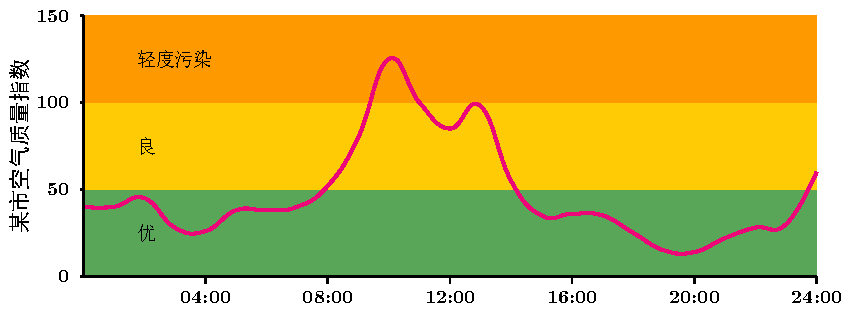
\includegraphics{Figures/aqi_pgf.pdf}
		\caption{}
	\end{figure}
	
	从图 3.1-1 中的曲线可知，\(t\) 的变化范围是数集 \(A_3 = \{t \mid 0 \leqslant t \leqslant 24\}\)，AQI 的值 \(I\) 都在数集 \(B_3 = \{I \mid 0 < I < 150\}\) 中. 对于数集 \(A_3\) 中的任一时刻 \(t\)，按照图 3.1-1 中曲线所给定的对应关系，在数集 \(B_3\) 中都有唯一确定的 AQI 的值 \(I\) 与它对应. 因此，这里的 \(I\) 是 \(t\) 的函数.
	
	\begin{thinkbox}[思考]
		你能根据图 3.1-1 找到中午 12 时的 AQI 的值吗？
	\end{thinkbox}
	
	\textcolor{blue}{\textbf{问题 4}} 国际上常用恩格尔系数 \(r\) (\(r = \frac{\text{食物支出金额}}{\text{总支出金额}} \times 100\%\)) 反映一个地区人民生活质量的高低，恩格尔系数越低，生活质量越高. 表 3.1-1 是我国某省城镇居民恩格尔系数变化情况，从中可以看出，该省城镇居民的生活质量越来越高.
	
	
	
	% ==================== 第三页 ====================
	\begin{table}[htbp]
		\centering
		\caption{表 3.1-1 我国某省城镇居民恩格尔系数变化情况}
		\renewcommand{\arraystretch}{1.3}
			\begin{tabular}{|c|c|c|c|c|c|c|c|c|c|c|}
			\hline
			年份 \(y\) & 2012 & 2013 & 2014 & 2015 & 2016 & 2017 & 2018	& 2019 & 2020 & 2021 \\ \hline
			恩格尔系数 \(r\) (\%) & 32.0 & 30.1 & 30.0 & 29.7 & 29.3 & 28.6 & 27.7 & 27.6 & 29.2 & 28.6 \\ \hline
		\end{tabular}
	\end{table}
	
	你认为按表 3.1-1 给出的对应关系，恩格尔系数 \(r\) 是年份 \(y\) 的函数吗？如果是，你会用怎样的语言来刻画这个函数？
	
	这里，\(y\) 的取值范围是数集 \(A_4 = \{20012, 2013, 2014, 2015, 2016, 2017, 2018, 2019, 2020, 2021\}\)；根据恩格尔系数的定义可知，\(r\) 的取值范围是数集 \(B_4 = \{r \mid 0 < r \leqslant 1\}\). 对于数集 \(A_4\) 中的任意一个年份 \(y\)，根据表 3.1-1 所给定的对应关系，在数集 \(B_4\) 中都有唯一确定的恩格尔系数 \(r\) 与之对应. 所以，\(r\) 是 \(y\) 的函数.
	
	\begin{summarybox}[归纳]
		上述问题 1\(\sim\)问题 4 中的函数有哪些共同特征？由此你能概括出函数概念的本质特征吗？
	\end{summarybox}
	
	上述问题的共同特征有：
	\begin{enumerate}[label=(\arabic*)]
		\item 都包含两个非空数集，用 \(A, B\) 来表示；
		\item 都有一个对应关系；
		\item 尽管对应关系的表示方法不同，但它们都有如下特性：对于数集 \(A\) 中的任意一个数 \(x\)，按照对应关系，在数集 \(B\) 中都有唯一确定的数 \(y\) 和它对应.
	\end{enumerate}
	
	事实上，除解析式、图象、表格外，还有其他表示对应关系的方法. 为了表示方便，我们引进符号 \(f\) 统一表示对应关系.
	
	一般地，设 \(A, B\) 是非空的实数集，如果对于集合 \(A\) 中的任意一个数 \(x\)，按照某种确定的对应关系 \(f\)，在集合 \(B\) 中都有唯一确定的数 \(y\) 和它对应，那么就称 \(f: A \to B\) 为从集合 \(A\) 到集合 \(B\) 的一个\textbf{函数}（function），记作
	\[
	y = f(x), \quad x \in A.
	\]
	其中，\(x\) 叫做自变量，\(x\) 的取值范围 \(A\) 叫做函数的\textbf{定义域}（domain）；与 \(x\) 的值相对应的 \(y\) 值叫做函数值，函数值的集合 \(\{f(x) \mid x \in A\}\) 叫做函数的\textbf{值域}（range）.
	
	显然，值域是集合 \(B\) 的子集. 在问题 1 与问题 2 中，值域就是 \(B_1\) 和 \(B_2\)；在问题 3 中，值域是数集 \(B_3\) 的真子集；在问题 4 中，值域 $C_4 =$ \{$0.3669$,$ 0.3681$,$ 0.3817$, $0.3569$, $0.3515$, $0.3353$, $0.3387$, $0.2989$, $0.2935$, $0.2857$\}，是数集 \(B_4 = \{r \mid 0 < r \leqslant 1\}\) 的真子集.
	
	\begin{thinkbox}[思考]
		17 世纪后期，德国数学家莱布尼茨第一次将“function”一词作为专门的数学术语；19 世纪，李善兰首次将 function 翻译成“函数”.
	\end{thinkbox}
	
	
	
	% ==================== 第四页 ====================
	我们所熟悉的一次函数 \(y = ax + b (a \neq 0)\) 的定义域是 \(\mathbf{R}\)，值域也是 \(\mathbf{R}\). 对应关系 \(f\) 把 \(\mathbf{R}\) 中的任意一个数 \(x\)，对应到 \(\mathbf{R}\) 中唯一确定的数 \(ax + b (a \neq 0)\).
	
	二次函数 \(y = ax^2 + bx + c (a \neq 0)\) 的定义域是 \(\mathbf{R}\)，值域是 \(B\). 当 \(a > 0\) 时，\(B = \left\{y \mid y \geqslant \frac{4ac - b^2}{4a}\right\}\)；当 \(a < 0\) 时，\(B = \left\{y \mid y \leqslant \frac{4ac - b^2}{4a}\right\}\). 对应关系 \(f\) 把 \(\mathbf{R}\) 中的任意一个数 \(x\)，对应到 \(B\) 中唯一确定的数 \(ax^2 + bx + c (a \neq 0)\).
	
	\begin{thinkbox}[思考]
		反比例函数 \(y = \frac{k}{x} (k \neq 0)\) 的定义域、对应关系和值域各是什么？请用函数定义描述这个函数.
	\end{thinkbox}
	
	\textcolor{blue}{\textbf{例 1}} 函数的解析式是舍弃问题的实际背景而抽象出来的，它所反映的两个量之间的对应关系，可以广泛地用于刻画一类事物中的变量关系和规律. 例如，正比例函数 \(y = kx (k \neq 0)\) 可以用来刻画匀速运动中路程与时间的关系、一定密度的物体的质量与体积的关系、圆的周长与半径的关系等.
	
	试构建一个问题情境，使其中的变量关系可以用解析式 \(y = x(10 - x)\) 来描述.
	
	\textbf{解：}把 \(y = x(10 - x)\) 看成二次函数，那么它的定义域是 \(\mathbf{R}\)，值域是 \(B = \{y \mid y \leqslant 25\}\). 对应关系 \(f\) 把 \(\mathbf{R}\) 中的任意一个数 \(x\)，对应到 \(B\) 中唯一确定的数 \(x(10 - x)\).
	
	如果对 \(x\) 的取值范围作出限制，例如 \(x \in \{x \mid 0 < x < 10\}\)，那么可以构建如下情境：
	
	长方形的周长为 20，设一边长为 \(x\)，面积为 \(y\)，那么 \(y = x(10 - x)\).
	
	其中，\(x\) 的取值范围是 \(A = \{x \mid 0 < x < 10\}\)，\(y\) 的取值范围是 \(B = \{y \mid 0 < y \leqslant 25\}\). 对应关系 \(f\) 把每一个长方形的边长 \(x\)，对应到唯一确定的面积 \(x(10 - x)\).
	
	\begin{summarybox}[探究]
		构建其他可用解析式 \(y = x(10 - x)\) 描述其中变量关系的问题情境.
	\end{summarybox}
	
	
	
	\subsection*{练习}
	1. 一枚炮弹发射后，经过 \(26\text{ s}\) 落到地面击中目标. 炮弹的射高为 \(845\text{ m}\)，且炮弹距地面的高度 \(h\)（单位：\(\text{m}\)）与时间 \(t\)（单位：\(\text{s}\)）的关系为
	\begin{equation}
		h = 130t - 5t^2. \tag{①}
	\end{equation}
	求①所表示的函数的值域与值域，并用函数的定义描述这个函数.
	
	
	
	% ==================== 第五页 ====================
	2. 2016 年 11 月 2 日 8 时至次日 8 时（次日的时间前加 0 表示）北京的温度走势如图所示.
	\begin{enumerate}[label=(\arabic*)]
		\item 求对应关系为图中曲线的函数的定义域与值域；
		\item 根据图象，求这一天 12 时所对应的温度.
	\end{enumerate}
	
	\begin{figure}[htbp]
		\centering
		% 此处为第 2 题图象的占位符，请替换为实际图片
		\framebox[0.8\textwidth]{\rule{0pt}{3cm} 第 2 题图象占位符}
		\caption{（第 2 题）}
	\end{figure}
	
	3. 集合 \(A, B\) 与对应关系 \(f\) 如下图所示：
	\begin{figure}[htbp]
		\centering
		% 此处为第 3 题图象的占位符，请替换为实际图片
		\framebox[0.6\textwidth]{\rule{0pt}{3cm} 第 3 题图象占位符}
		\caption{（第 3 题）}
	\end{figure}
	
	\(f: A \to B\) 是否为从集合 \(A\) 到集合 \(B\) 的函数？如果是，那么定义域、值域与对应关系各是什么？
	
	4. 构建一个问题情境，使其中的变量关系能用解析式 \(y = \sqrt{x}\) 来描述.
	
\end{document}